\documentclass[]{article}
\newcommand{\FileDepth}{../../..}
\usepackage[letterpaper, landscape, margin=0.5cm]{geometry}
\usepackage[T1]{fontenc}
\usepackage{textcomp}%Not strictly necessary, but gives \textmu command for "micro."
\usepackage{fancyhdr}
\usepackage{amsmath}
\usepackage{amssymb}
\usepackage{graphicx}
\usepackage{xcolor}
\usepackage{tikz}
\usetikzlibrary{calc}
\usepackage{censor}
\usepackage{hyperref}
%opening
\newcommand{\SecType}{L}
\newcommand{\Lec}{1}
\title{PH 21X Lecture \Lec}
\author{Benjamin Bauml}
\date{Term 2024}

\newcommand{\Purpose}{4}
\newcommand{\DefOnly}{0}

% Version 2024-06-14
% Changes
% 2024-02-21 Added xstring package to enable smooth implementation of new \ModePage command.
% 2024-04-27 Set up to split activities and formatting aspects into separate files. Removed dependence on xcomment. Added an automatic counter to number the activities in a problem set.
% 2024-05-19 Revised old format for \TeachingTips command, which did not support \DefOnly.
% 2024-06-14 Added Repurpose environment to allow mixing of different purpose levels in the same document.
\usepackage{tcolorbox}
\usepackage{xstring}
% You will want the following four lines in your document (the last two uncommented):
% For Assignment, leave Purpose as 1. For Worksheet, set to 2. For Student Solution, set to 3. For Teacher Solution, set to 4.
% If you want keep the pieces from being called manually, set DefOnly to 0.
%\newcommand{\Purpose}{4}
%\newcommand{\DefOnly}{1}
\newcommand{\Exclusion}{0}
\newcommand{\PageTurn}{0}
\newcommand{\GrayProb}{0}
\newcommand{\Tipsy}{0}

% Assignment
\if\Purpose1
\renewcommand{\Exclusion}{1}
\fi
% Worksheet
\if\Purpose2
\renewcommand{\Exclusion}{1}
\renewcommand{\PageTurn}{1}
\fi
% Student Solution
\if\Purpose3
\renewcommand{\PageTurn}{1}
\renewcommand{\GrayProb}{1}
\fi
% Teaching Copy
\if\Purpose4
\renewcommand{\PageTurn}{1}
\renewcommand{\GrayProb}{1}
\renewcommand{\Tipsy}{1}
\fi

\newenvironment{Repurpose}[1]{
\renewcommand{\Purpose}{#1}
\renewcommand{\Exclusion}{0}
\renewcommand{\PageTurn}{0}
\renewcommand{\GrayProb}{0}
\renewcommand{\Tipsy}{0}
% Assignment
\if\Purpose1
\renewcommand{\Exclusion}{1}
\fi
% Worksheet
\if\Purpose2
\renewcommand{\Exclusion}{1}
\renewcommand{\PageTurn}{1}
\fi
% Student Solution
\if\Purpose3
\renewcommand{\PageTurn}{1}
\renewcommand{\GrayProb}{1}
\fi
% Teaching Copy
\if\Purpose4
\renewcommand{\PageTurn}{1}
\renewcommand{\GrayProb}{1}
\renewcommand{\Tipsy}{1}
\fi
}{}

\def \NewQ {0}
\def \PForce {0}
\newcommand{\MaybePage}[1]{
	\def \PForce {#1}
	\if\PForce1
	\newpage
	\else
	\if\NewQ0
	\gdef \NewQ {\PageTurn}
	\else
	\newpage
	\fi
	\fi
}

\newcommand{\ModePage}[1]{
	\IfSubStr{#1}{\Purpose}{\newpage}{}
}

\newcounter{ActNumber}
\setcounter{ActNumber}{0}

\newcommand{\Problem}[4][0]{%The first argument is optional, and if it is set to 1, the \newpage will be forced. The second argument is the name of the activity, the third is the command the activity is stored as, and the fourth is the actual problem statement.
\newcommand{#3}{
\MaybePage{#1}
\addtocounter{ActNumber}{1}
\section*{\SecType\Week-\theActNumber: #2}
\if\GrayProb1
\begin{tcolorbox}[colback=lightgray,colframe=lightgray,sharp corners,boxsep=1pt,left=0pt,right=0pt,top=0pt,bottom=0pt,after skip=2pt]
\else
\begin{tcolorbox}[colback=white,colframe=white,sharp corners,boxsep=1pt,left=0pt,right=0pt,top=0pt,bottom=0pt,after skip=2pt]
\fi
#4
\end{tcolorbox}\noindent
}
\if\DefOnly0
\else
#3
\fi
}
	
\newcommand{\ProblemSub}[3][0]{%The first argument is optional, and if a string of numbers is entered into it, it will force a \newpage in any \Purpose that shows up in the string. For example, "13" would lead to the newpage being forced in modes 1 and 3. The second is the command the activity is stored as, and the third is the actual problem statement.
\newcommand{#2}{
\ModePage{#1}
\if\GrayProb1
\begin{tcolorbox}[colback=lightgray,colframe=lightgray,sharp corners,boxsep=1pt,left=0pt,right=0pt,top=0pt,bottom=0pt,after skip=2pt]
\else
\begin{tcolorbox}[colback=white,colframe=white,sharp corners,boxsep=1pt,left=0pt,right=0pt,top=0pt,bottom=0pt,after skip=2pt]
\fi
#3
\end{tcolorbox}\noindent
}
\if\DefOnly0
\else
#2
\fi
}
		
\newcommand{\Solution}[2]{%The first argument is the command the solution is stored as, and the second is the actual solution.
\newcommand{#1}{
\if\Exclusion0
#2
\fi
}
\if\DefOnly0
\else
#1
\fi
}
		
\newcommand{\ProblemFig}[2]{%The first argument is the command the figure is stored as, and the second is the actual figure.
\newcommand{#1}{
\begin{figure}[h]
#2
\end{figure}
}
\if\DefOnly0
\else
#1
\fi
}

\newcommand{\TeachingTips}[2]{%The first argument is the command the tip is stored as, and the second is the actual tip.
\newcommand{#1}{
\if\Tipsy1
\begin{tcolorbox}[colback=lightgray,colframe=black]
#2
\end{tcolorbox}
\fi
}
\if\DefOnly0
\else
#1
\fi
}
\usepackage[absolute]{textpos}
% This package relies on Assignment Format 2024-06-14 or later to work. It is recommended that the Purpose and DefOnly commands be given as such:
%\newcommand{\Purpose}{4}
%\newcommand{\DefOnly}{0}
% Activities need to be entered outside of the TeacherMargin and PresentSpace environments, otherwise they will be defined only locally. They can even go in the preamble.
\newenvironment{TeacherMargin}{\begin{textblock*}{10.8cm}(0.5cm,0.5cm)
\small}{\end{textblock*}
\hspace{0.1cm}}
\newenvironment{PresentSpace}{\begin{textblock*}{0.3cm}(26.85cm,9.35cm)
--
\end{textblock*}
\begin{textblock*}{0.3cm}(26.85cm,18.7cm)
--
\end{textblock*}
\begin{textblock*}{0.3cm}(26.85cm,12.24cm)
	--
\end{textblock*}
\begin{textblock*}{15.6cm}(11.8cm,0.5cm)
\begin{Repurpose}{1}
\Large}{\end{Repurpose}
\end{textblock*}
\hspace{0.1cm}}

%\newcommand{\FBDaxes}[3]{
	\begin{scope}[shift={(#1)},rotate=#2]
		% x-axis
		\draw[thick,->] (-2,0) -- (2,0);
		\node[anchor=west] at (2,0) {$x$};
		% y-axis
		\draw[thick,->] (0,-2) -- (0,2);
		\node[anchor=west] at (0,2) {$y$};
		\coordinate (#3) at (0,0);
	\end{scope}
}
\newcommand{\FBDvectorMA}[4]{
	\begin{scope}[shift={(#1)}]
		\coordinate (#4tip) at ({#2*cos(#3)},{#2*sin(#3)});
		\draw[ultra thick,blue,->] (#1) -- (#4tip);
	\end{scope}
}
\newcommand{\FBDvectorXY}[3]{
	\begin{scope}[shift={(#1)}]
		\coordinate (#3tip) at (#2);
		\draw[ultra thick,blue,->] (0,0) -- (#3tip);
	\end{scope}
}
\newcommand{\FBDdot}[1]{
	\filldraw[black] (#1) circle (3pt);
}
%\newcommand{\MVec}[3][0]{%Creates a momentum vector of length #3 centered at #2 and rotated #1 degrees counterclockwise.
	\begin{scope}[rotate=#1,shift={(#2)}]
		\draw[->,thick] ({-#3/2},0) -- ({#3/2},0);
	\end{scope}
}
\newcommand{\MDot}[1]{%Creates a dot at #1 to represent a zero vector.
	\filldraw (#1) circle (1pt);
}
\newcommand{\MVDRows}[2][4.5]{%Creates the rows (initial, delta, final) of a momentum vector diagram. The optional argument determines the width of the table, and defaults to a good length for three columns (two objects and the total system). The non-optional argument gives a coordinate name (not displayed) to the diagram.
	\begin{scope}
		%\draw[thick] (0,5.5) -- (0,0);
		\draw[thick] (-1,4.5) -- (#1,4.5);
		\node at (-0.5,3.75) {$\vec{p}_{i}$};
		\draw[thick] (-1,3) -- (#1,3);
		\node at (-0.5,2.25) {$\Delta\vec{p}$};
		\draw[thick] (-1,1.5) -- (#1,1.5);
		\node at (-0.5,0.75) {$\vec{p}_{f}$};
		\coordinate (#2) at (0,5);
	\end{scope}
}
\newcommand{\MVDCol}[4][0.75]{%Creates a column for an object in a momentum vector diagram. The first (non-optional) argument is the coordinate name (not displayed) of the column, while the second is the displayed column header. The first argument also names the three entries down the column. The third argument anchors the column, so it should either be the coordinate name of the MVD (for the first column) or the coordinate name of the previous column. The optional argument indicates how far the center of the column should be from the previous column's edge, and defaults to 0.75
	\begin{scope}[shift={(#4)}]
		\node at (#1,0) {#3};
		%\draw[thick] ({#1*2},0.5) -- ({#1*2},-5);
		\draw[thick] (0,0.5) -- (0,-5);
		\coordinate (#2init) at (#1,-1.25);
		\coordinate (#2delt) at (#1,-2.75);
		\coordinate (#2fin) at (#1,-4.25);
		\coordinate (#2) at ({#1*2},0);
	\end{scope}
}

%\input{\FileDepth/Activities/Activity_One/Activity_One.tex}
%\input{\FileDepth/Activities/Activity_Two/Activity_Two.tex}

\begin{document}
\begin{TeacherMargin}
\noindent\textbf{Meetings with Benjamin}

There are two surveys on Canvas in the Start Here module. Only do the one associated with your lab section. These surveys will help me determine when to schedule my regular drop-in and appointment hours most effectively.

\noindent\textbf{Meetings with the TAs}

The Wormhole is the central place in the Physics Department to get help on homework. It is on the third floor of Weniger Hall, in room 334, and it will be open 2-5pm Monday through Thursday, 10am-5pm on Fridays. Not all of the TAs in the Wormhole are on the teaching team for this course, but they can all help you with physics assignments.
\end{TeacherMargin}
\begin{PresentSpace}
\begin{center}
	\huge Welcome to PH 211!
\end{center}
\noindent\textbf{Instructor:} Benjamin Bauml

\noindent\textbf{Drop-In and Appointment Hours:} To Be Determined (TBD)

To book an individual appointment with me, see my \href{https://outlook.office.com/bookwithme/user/8a879d0af7bf45e890abd3d888d8bfe4@oregonstate.edu?anonymous&ep=plink}{\color{blue}Booking Page}. \\

\noindent\textbf{Teaching Assistants (TAs):}

\noindent Kevin Dimmitt (Tuesday lab) and Ben Hansen (Wednesday lab)

\noindent\textbf{\href{https://wormhole.physics.oregonstate.edu/}{\color{blue}Wormhole} Hours:} Fridays

10 a.m. - 12 p.m. (Kevin)

1 p.m. to 3 p.m. (Ben) \\

\noindent\textbf{Learning Assistants (LAs):}

\noindent Austin Gugenheim, Matilda Pike, Ahmed Rashid
\end{PresentSpace}
\newpage
\begin{TeacherMargin}
\noindent\textbf{What is identity?}

In social science, identity consists of traits that characterize a person, and these traits can be of various sorts and come from various aspects of one's life.

For instance, I get certain aspects of my identity from my job. I think of myself as a physicist, a mathematician, and a teacher.

I also get identity from my hobbies, interests, and preferences. I like to dance, play music and games, and write. I like cats. These traits can make up part of my identity as well.

Identity can come from personal or societal sources as well, such as gender identity, national identity, ethnic identity, religious identity, political identity, and so on. A lot of these can be very personal, so you don't need to feel compelled to share them with me. Note that I blacked out one of my identities, because while I felt it was important, I didn't feel like sharing it at this time.

\noindent\textbf{Priorities}

Of course you have a life outside of this class! You should expect to put in time and hard work to keep up with the class, and you will need to balance your obligations to this class against your other responsibilities and interests. I absolutely don't expect you to sacrifice everything for this class, but I do expect you to take it seriously and put in effort.

Your instructional team has other priorities as well. The TAs and I have research obligations to attend to that will occupy some of our time. Some of us have families to care for. We also have hobbies that help us refresh ourselves. For instance, I am definitely not missing an opportunity to dance Argentine tango tomorrow.

That said, we are here to help you learn, and we will be putting a great deal of effort into that. You are a significant priority for us.

\begin{center}
	\Large The Getting to Know You assignment is due Friday. The online component is due at 8:00 p.m.
\end{center}
\end{TeacherMargin}
\begin{PresentSpace}
\begin{center}
	\textbf{Getting to Know You}
\end{center}
\textbf{What is your preferred full name?}
{\color{blue}\hrule}
\begin{center}
	Benjamin No\"{e} Bauml
\end{center}
\textbf{What do you want me to call you?}
{\color{blue}\hrule}
\begin{center}
	You may call me Benjamin.
	
	If you don't want to call me by my first name, you may call me Mr. Bauml.
\end{center}
\textbf{What are your preferred pronouns?}
{\color{blue}\hrule}
\begin{center}
	He/Him/His
\end{center}
\textbf{What identities do you associate with yourself? Include any that you feel are important to who you are, and that you are comfortable sharing with me.}
{\color{blue}\hrule}
\begin{center}
	Physicist, Mathematician, Teacher, Social Dancer, Musician, Gamer, Writer, Cat Person, \censor{Bisexual}
\end{center}
\textbf{What are your interests? What do you want to learn? What do you do for fun?}
{\color{blue}\hrule}
\vspace{10pt}

\noindent\textbf{Aside from this class, what are your priorities for the term? What goals (educational, professional, personal) do you have during this time?}
{\color{blue}\hrule}
\vspace{10pt}

\noindent\textbf{Where does this class rank among your priorities for the term? If it helps, you can rank it twice; where would you rank it in terms of its actual importance to you, and where do you think it needs to be ranked in your priorities for you to be successful?}
{\color{blue}\hrule}
\vspace{10pt}

\noindent\textbf{What is your major? What year in college is this for you? What are you studying to do?}
{\color{blue}\hrule}
\vspace{2pt}
\end{PresentSpace}
%\newpage
\begin{comment}
	Instructor Notes
\end{comment}
\begin{comment}
\begin{center}
	\textbf{Getting to Know You}
\end{center}
\textbf{What are your interests? What do you want to learn? What do you do for fun?}
{\color{blue}\hrule}
\vspace{2pt}
I am an avid dancer, with interest in ballroom dance, swing, and Argentine tango.

I enjoy games, especially roleplaying games, such as \textit{Dungeons \& Dragons} (especially revised 3rd edition) and \textit{Call of Cthulhu}.

I have played the French horn since 5th grade, and I have some experience with piano, baritone ukulele, and Native American flute. I am early in the process of teaching myself to play the English concertina.

I like to read fantasy and science fiction, and I have some interest in creative writing.

I took German for three years in high school.

My research in physics has been focused on quantum mechanics. My undergraduate research focused on the consistent histories formulation, and my graduate research so far has focused on weak measurement. I find quantum computation and cryptography interesting, but I am not really in a position to change my research direction to those topics at this time.

\noindent\textbf{Aside from this class, what are your priorities for the term? What goals (educational, professional, personal) do you have during this time?}
{\color{blue}\hrule}
\vspace{2pt}

\noindent\textbf{Where does this class rank among your priorities for the term? If it helps, you can rank it twice; where would you rank it in terms of its actual importance to you, and where do you think it needs to be ranked in your priorities for you to be successful?}
{\color{blue}\hrule}
\vspace{2pt}

\noindent\textbf{What is your major? What year in college is this for you? What are you studying to do?}
{\color{blue}\hrule}
\vspace{2pt}
\end{comment}
\newpage
\begin{TeacherMargin}
\noindent\textbf{Playing Cards}

Sharpie-like, felt tip, gel, or calligraphy pens are probably the best for this. The texture of a playing card does not work well with pencils or ballpoint pens. Some dry erase markers will leave good marks, but others will wipe away easily.

I plan on using these to randomize groups and perhaps to call on people randomly. If I call on you at random, don't panic. I won't make you answer if you don't want to. I encourage you to ask a clarifying question if you don't have an answer, as it will help you and your classmates learn (and it will help me know what I need to make clearer to help you learn), but I also won't make you ask a question if you don't want to.

I would like to keep these to remember you by, but if you feel really strongly about getting these back, you can ask at the end of the term.
\end{TeacherMargin}
\begin{PresentSpace}
\begin{center}
	\textbf{Getting to Know You -- In-Class Submission}
\end{center}
Write your preferred full name and pronouns on a blank playing card, along with any other drawings you want to add.

\noindent These should be turned in during Friday's lecture. \\
\begin{figure}[h]
	\centering
	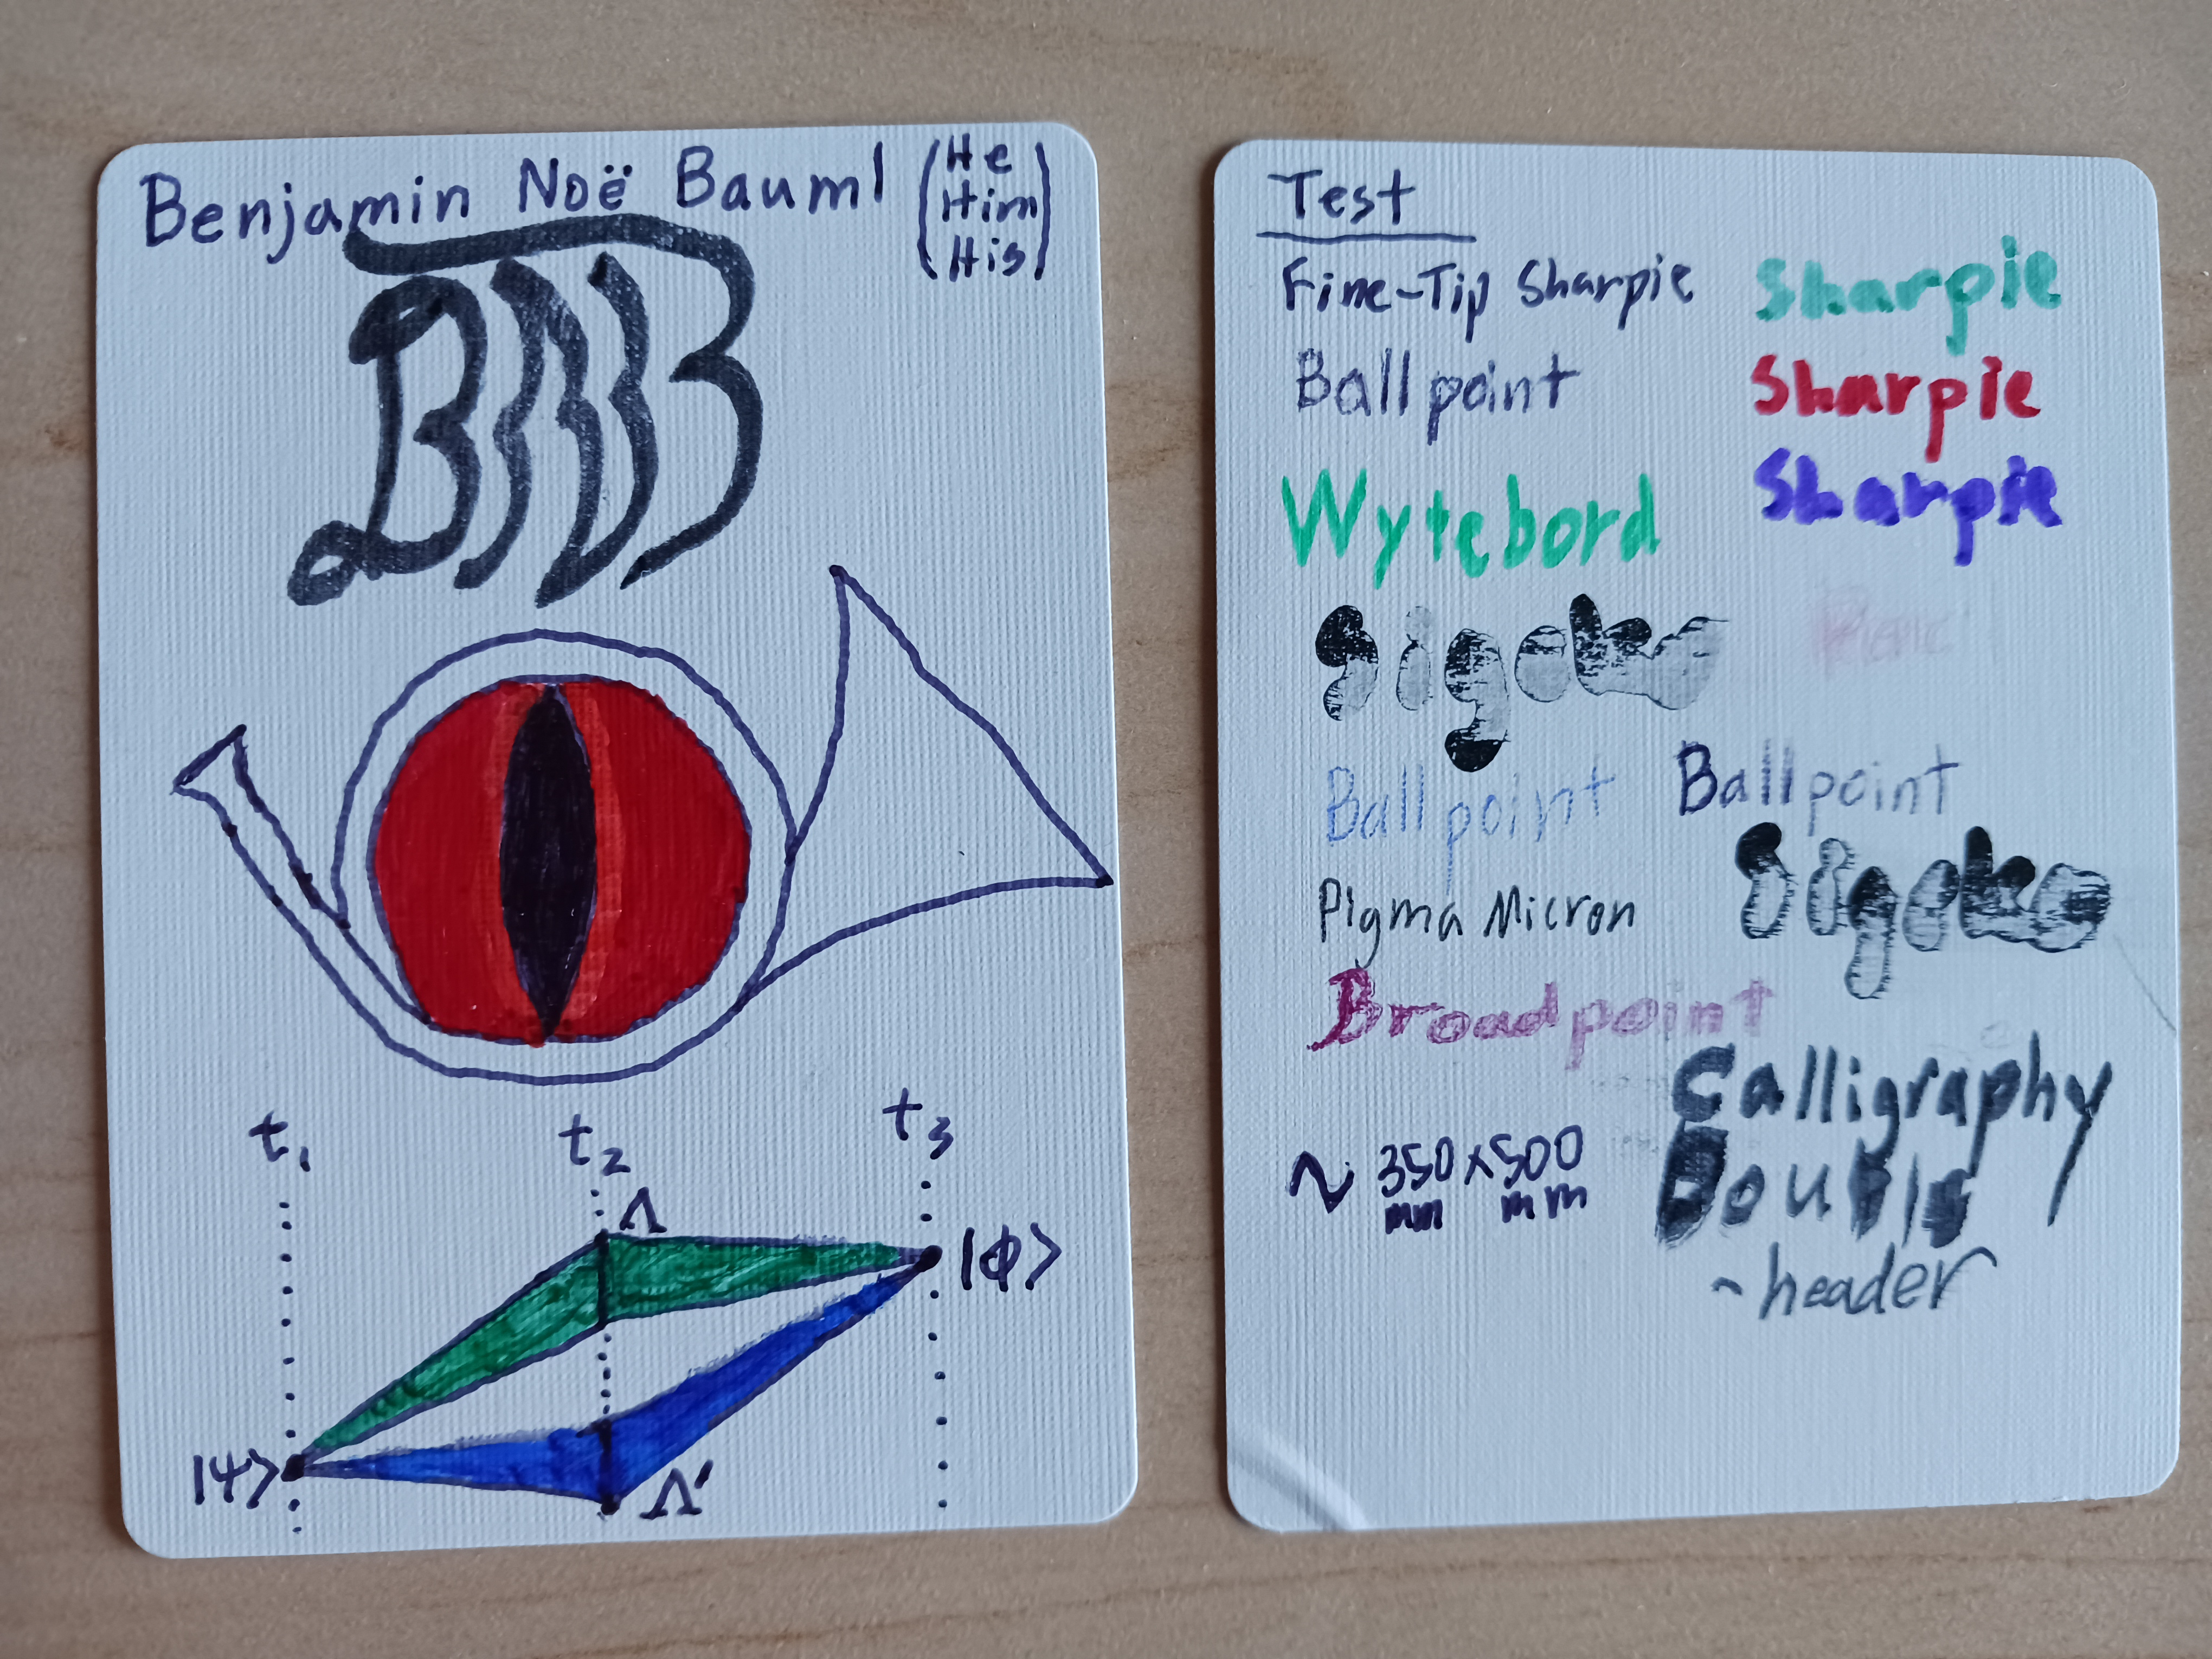
\includegraphics[scale=0.1]{PlayingCards}
\end{figure}
\end{PresentSpace}
\newpage
\begin{TeacherMargin}
%\footnotesize
\noindent\textbf{Lecture and Studio} The science of thinking informs the structure for this course. Lecture and studio will consist largely of activities meant to stimulate your thinking in the course. It is critically important to be present and engaged in lecture and studio every week.

Everyone's learning will suffer if illness spreads through our classroom. If you are sick, stay home and look over the posted lecture slides; work through the activities on your own. Notes from class will be posted later for you to see, and you can email me questions.

You will be working in groups in lecture. For the first couple of weeks, I will randomize the groups so you can meet as many of your classmates as possible. At the end of week two, you will be choosing your groups for your projects, and you will mostly be grouped with them in class after that. We will talk more about the projects later, but for now, focus on thinking about whom you might want to work with.

\noindent\textbf{Get-Ready Activities} You will be introduced to content in the Get-Ready activities. It is alright to make mistakes and be confused at first. Write down any questions you have so you remember to ask about them in lecture! We will be exploring activities to get deeper into the content in lecture and studio, so it is critical that you do the Get-Ready activities beforehand.

Currently, Get-Ready activities are submitted after lecture. That way, you can add notes based on what you learned in lecture and add any new questions that arise from lecture. However, if it becomes apparent that the readings are not being done before lecture, I reserve the right to change this policy so that notes from Get-Ready activities must be turned in before lecture as well.

\noindent\textbf{Lab} Lab is an important experiential learning opportunity that will introduce you to proper experimental procedure, working with uncertainty in measurements, and clear scientific communication. There are six labs to do, and each one has an important lesson, so we want you to complete all six labs.

The last lab will run in Week 7, and in Week 8, the lab rooms will be open at their scheduled times for make-up labs. If you missed one lab, you can attend one of the two sections to make it up. If you missed two, you will need to attend both sections to make up both labs. If you missed three, or cannot make it to both sections to complete two missed labs, come talk to me about your options.

\noindent\textbf{Homework} Homework problems will challenge you to really deepen your understanding of the content. There are two main formats that problems follow: \href{https://lipa.physics.oregonstate.edu/sec_what-is-motion.html}{\color{blue}Explanations} and \href{https://lipa.physics.oregonstate.edu/sec_real-world-context.html}{ARCS}. Both are in the online textbook and in Canvas. These formats are not just to help the instructional team follow your reasoning, but they train you to complete important steps in breaking down and explaining problems.

You are encouraged to work together to understand the homework. However, the work you submit should be your own. It is not acceptable to copy someone else's work. If you work with someone, you need to write down their name and acknowledge that you worked together. Giving proper credit to collaborators is extremely important, particularly in science.

Most assignments will be submitted through Canvas. Labs and other group assignments will be submitted through Gradescope, which you will learn more about in lab. If you continue on to PH 212, you will turn \textbf{everything} in on Gradescope, so you should get familiar with it now.

\noindent\textbf{Quiz} We also have plans to have an in-class quiz on Monday of Week 4.
\end{TeacherMargin}
\begin{PresentSpace}
\begin{center}
	\textbf{Science of Thinking}
\end{center}
Before class, I asked you to watch a video on the Science of Thinking. \\

\noindent Talk with your neighbor about something you learned from the video.
\vspace{0.5cm}
%\vspace{5.5cm}
\begin{center}
	\textbf{Course Structure}
\end{center}
\noindent\textbf{Lecture and Studio}
\begin{itemize}
\item Time to practice the content; opportunity to ask questions; group work!
\item Attendance and participation in lecture/studio is critical to learning in this course! (But stay home if you are sick; lecture slides will be posted to Canvas, and you can feel free to email me any questions you have. We will work with you to help you keep up!)
\end{itemize}
\noindent\textbf{Get-Ready Activities}
\begin{itemize}
	\item Readings, videos, and exercises to complete \textbf{before} Monday and Wednesday lectures.
	\item Add notes based on lecture/studio and submit by the end of the day.
	\item Prominently write questions you have about the reading and from lecture. We want to know what you are wondering about!
\end{itemize}
\noindent\textbf{Lab}
\begin{itemize}
	\item Opportunities to make up one or two missed labs in the last week.
	\item If you cannot complete all labs, talk to me about your options.
\end{itemize}
\noindent\textbf{Homework}
\begin{itemize}
	\item Due at 10 p.m. on Fridays.
	\item You may work with others, but \textbf{you must include their names} on your submission, and your \textbf{submitted work must be your own}, not a copy of someone else's work.
\end{itemize}
\end{PresentSpace}
\newpage
\begin{TeacherMargin}
\noindent\textbf{Excerpt from \textit{Ungrading}, edited by Susan D. Blum}

Several years ago I encountered the work of Dylan Wiliam, who researched the effect of teacher feedback on student improvement. In his book \textit{Embedded Formative Assessment}, he cites a study by Ruth Butler wherein she examines the three types of feedback teachers give: grades alone, both grades and comments, and comments alone.

The results of Butler's research might seem counterintuitive: the students who showed the most growth were those who received comments alone. Even grades paired with comments---which at face value would seem to be the richest form of feedback---were just as ineffective as giving grades alone.

Wiliam concludes: ``That most students virtually ignore \dots painstaking correction, advice, and praise is one of public education's best-kept secrets.''

Not only do grades not encourage growth, they inhibit it. Grades take the focus off feedback.
\begin{flushright}
	---Arthur Chiaravalli
	
	\textit{Ungrading} Chapter 5
\end{flushright}
\end{TeacherMargin}
\begin{PresentSpace}
\begin{center}
	\textbf{Ungrading Policy}
\end{center}
\textbf{You will not receive grades on individual assignments.}
\begin{itemize}
	\item You will receive feedback to help you think about your learning and improve your work.
	\item There is no direct calculation from the points for completion and attendance in Canvas to your overall grade.
\end{itemize}
\textbf{You will propose your own final grade.}
\begin{itemize}
	\item As your final assignment of the term, you will write a reflection on your learning and your work and decide what grade you have earned.
	\item Attendance, participation, and assignments factor into the proposal.
	\item I have the right to change the grade you propose.
\end{itemize}
\textbf{You will get to practice before the final ungrading.}
\begin{itemize}
	\item At the end of Week 4, you will get to go through the ungrading process based on the work you have completed so far. If you have trouble assessing your own learning at this point, we will help fix any issues and prepare you for the final ungrading.
	\item There are small reflections on learning at the end of each homework assignment.
\end{itemize}
\end{PresentSpace}
\newpage
\begin{TeacherMargin}
\noindent I think physics is \dots
\begin{itemize}
	\item Collaborative \\ Physicists often work together to push the boundaries of knowledge. They trade ideas and try to find the answers to questions together. Even when working alone, a physicist is building on knowledge discovered by others.
	\item Challenging \\ We need to develop our skill at examining physical situations, simplifying them, applying math to them, and recognizing the key concepts that are involved. There is a lot of translation, calculation, and interpretation.
	\item Cumulative \\ New concepts build on old concepts at every step. Really interesting things can be discovered when tools from different areas are brought to a problem so it can be investigated in a new way.
	\item Conceptual \textbf{and} Quantitative \\ We don't just calculate things and report numbers, though there is certainly a great deal of math we must do. We are also trying to understand the world better, and that means familiarizing ourselves with conceptual information about how the world works and building (and often rebuilding) our physical intuition.
\end{itemize}
\end{TeacherMargin}
\begin{PresentSpace}
\begin{center}
	\textbf{What is physics?}
\end{center}
Come up with a sentence (or two) for each of the following questions:
\begin{itemize}
	\item What is physics?
	\item What do you expect to learn from physics?
\end{itemize}
If someone asked you to describe physics using \underline{one word}, what would you choose?
\end{PresentSpace}
\newpage
\begin{TeacherMargin}
\noindent\textbf{Motion}

We will examine how objects move through space.

\noindent\textbf{Forces}

We will describe how objects interact with each other by pushing and pulling.

\noindent\textbf{Energy}

We will talk about different forms of energy and how they transform, and how energy affects objects.

\noindent\textbf{Momentum}

We will take another perspective on changing the motion of objects, with a focus on collisions and explosions.

\end{TeacherMargin}
\begin{PresentSpace}
\begin{center}
	\textbf{Course Context}
\end{center}
The physical contexts we will study are:
\begin{itemize}
	\item Motion
	\item Forces
	\item Energy
	\item Momentum
\end{itemize}
\vspace{3cm}
\begin{center}
	\textbf{What is motion?}
\end{center}
\begin{itemize}
	\item Write down something you know about \textbf{motion}.
	\item Turn to your neighbor and talk about what you each know.
	\item Find another neighbor and talk about what you each know.
	\item We will be building a model for describing the \textit{\textbf{motion}} of \textit{\textbf{objects}}.
\end{itemize}
\end{PresentSpace}
\newpage
\begin{TeacherMargin}
Isaac Newton hypothesized that the force which kept celestial bodies in orbit was the force that caused objects to fall. He developed a theory of universal gravitation that explained earlier empirical observations of the motion of planets.

Newtonian gravity is not perfect, but it is a good approximation to the world around us for most practical purposes. Albert Einstein's theory of general relativity (GR) explains such things as the effect of gravity on the flow of time and the shape of space. Plenty of modern experiments (such as gravitational wave astronomy) are currently testing its limits to see if we can find anything not explained by GR.

We get a better understanding of the world around us by breaking and revising models!

If you are concerned that you are not as smart as Newton and Einstein, don't worry. The average physicist is not nearly as smart as either of them, but can still make significant contributions to our knowledge of the world. There is an unfortunate mythology around physics that it is advanced by solitary geniuses, but remember, physics is \textbf{collaborative} and \textbf{cumulative}, built from many normal people working together and building on what came before.
\end{TeacherMargin}
\begin{PresentSpace}
\begin{center}
	\textbf{Model Building}
\end{center}
How do physicists do physics?
\begin{itemize}
	\item Make an observation
	\item Take data
	\item Come up with a model that explains the observation
	\item Test the model
	\item Repeat
\end{itemize}
The models we come up with will help us describe what we see around us!
\begin{figure}[h]
	\centering
	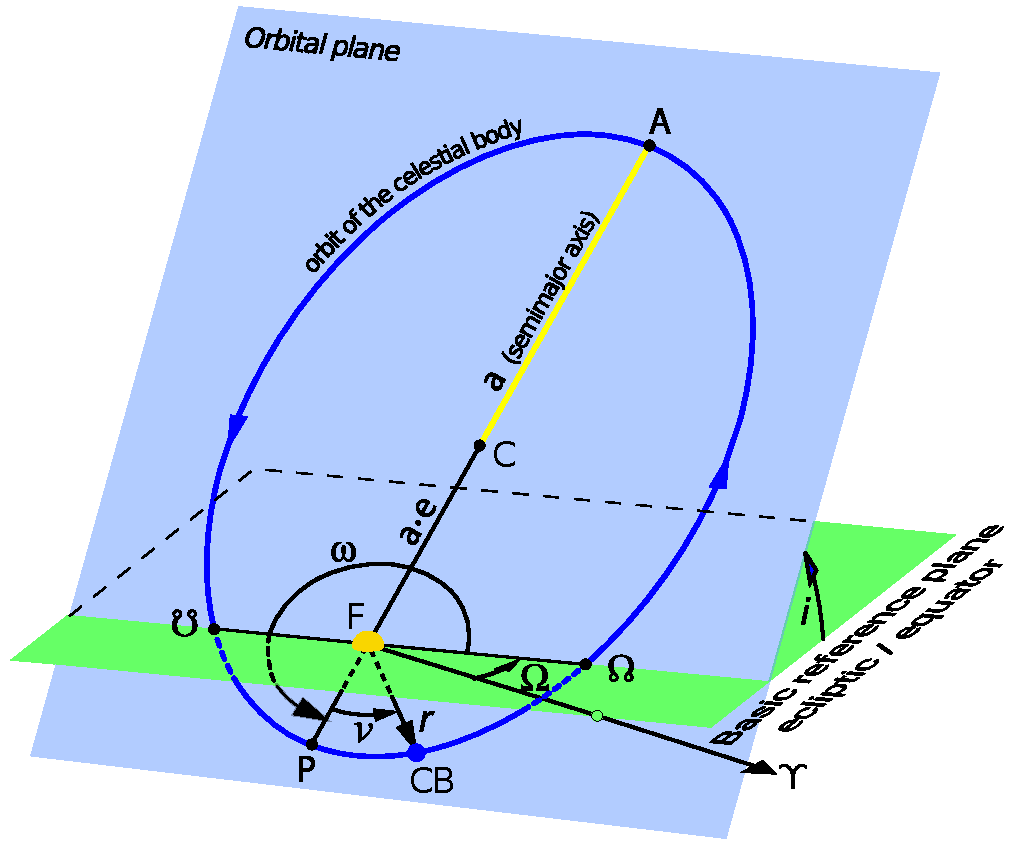
\includegraphics[scale=0.4]{BahnelementeEllipse_eng.pdf}
\end{figure}

\begin{center}
	\small Wikimedia Commons user Mliu92, released under CC-BY 4.0
\end{center}

\begin{figure}[h]
	\centering
	
\includegraphics[scale=0.4]{J0806.jpeg}
\end{figure}

\begin{center}
	\small Credit: Tod Strohmayer (GSFC), CXC, NASA - Illustration: Dana Berry (CXC)
\end{center}
\end{PresentSpace}
\newpage
\begin{TeacherMargin}
\noindent\textbf{Respect}

This goes in all directions. Students need to respect each other---you are all learning the content, you each have your own pace, and you all will make mistakes. Students need to respect the instructional team, which is here to help, and the instructional team needs to respect the students. If you ever feel that you are not being respected, please tell us so we can try to resolve the issue.

When I gather the entire class' attention to go over a concept or activity, noise and side conversations need to be kept to a minimum. If people talk over me, they are disrespecting me and those who are trying to listen to me. Even if I address an individual student, or if I stop talking to let a student talk instead, that does not mean you can stop giving your attention. It is disrespectful to the student who is trying to talk, as well as to me and anyone else trying to listen. The thoughts and questions of your classmates are just as important as mine.

\noindent\textbf{Doing and Questioning}

Remember, our class structure is build around active engagement, and you will not be getting the most out of this learning experience if you do not stay engaged with the activities and ask questions to deepen your understanding.

\noindent\textbf{Making Sense}

One of the most valuable skills we will learn is making sense of answers. Some day, you will be doing something for which there is not an answer key for reference, and you will need to be able to evaluate your own answer to determine whether or not it is reasonable.

Another problem with scientific jargon is that we will often use words from regular speech in very specific ways. For example, energy and power are sometimes used interchangeably in conversation, but in physics, they mean very specific, distinct things.

You will be generating a lot of your own representations. It is important to develop skill with making representations clear and informational, with enough annotation that you can organize a problem around your representations.
\end{TeacherMargin}
\begin{PresentSpace}
\begin{center}
	\textbf{Principles for Success}
\end{center}
\textbf{Treat everyone with respect.}
\begin{itemize}
	\item Everyone's ideas matter.
	\item Act professionally.
\end{itemize}
\textbf{Learn by doing and questioning.}
\begin{itemize}
	\item Everyone in your group is responsible for participating and working together.
\end{itemize}
\textbf{Make sense of everything.}
\begin{itemize}
	\item Jargon alert -- if you hear a term you don't understand, ask!
	\item Representations -- if you don't understand what a picture or image is showing, ask!
\end{itemize}
\end{PresentSpace}
\end{document}